\par Calorimeters are detectors in particle and nuclear physics that measure the
energy of particles by inevitably absorbing all  
of the particle's energy and converting it into heat. This absorption can be through 
scintillation, ionization or cherenkov radiation, among several other options through which  
the candidate particle can interact with matter. Scintillation and ionization are most commonly used to detect 
high energy particles. 

\par For scintillation the candidate particle excites electrons that are subsequently 
de-excited, emitting photons which are multiplied and turned into signal. Detectors 
in which the electrons are excited from molecules are known as organic scintillators, 
while those in which the electrons are excited from atoms are called 
inorganic scintillators. Inorganic scintillators tend to have a higher photon yield than 
organic scintillators so they are widely used in high energy experiments. Organic scintillators 
are therefore outside the scope of this thesis. For inorganic scintillators, 
the atomic medium is a high density crystal of low cost material. Electrons in 
the valence state are excited by the ionizing particle to a conduction state,
 leaving a hole in the valence state. Upon de-excitation, a photon is emitted and 
is turned into signal. To minimize the de-excitation response time impurities whose energy levels lie between 
the valence band and the conduction band are added to the material. This offers the 
excited electrons a faster de-excitation option, drastically improving the detector 
time resolution. For ionization detectors on the other hand, electrons 
on average rarely get de-excited from the conduction state. Rather, they are collected 
and the resultant current is turned into signal.   

\par In the ionization case, excited electrons are in general so energetic that they further interact with matter, 
producing secondary and tertiary particles that in turn produce other particles of lower energy. This creates a 
particle shower whose shape can be studied to reconstruct the original particle energy.
 The primary interaction of electrons and matter at high energy is
primarily through deflection by atomic nuclei, emitting 
photons which in turn decay into an positron-electron (\epem) pair. The \epem\ pair in turn interacts 
similarly, producing even more \epem\ pairs until their energies are below an energy 
where the main form of dissipation is ionization and excitation rather than the 
creation of other particles. A particle shower initiated by leptons and photons through 
electromagnetic processes is known as an electromagnetic (EM) shower, and the medium of the calorimeter 
in which it develops is known as an absorber. The EM shower depth is characterized by 
a property of the absorber called radiation length $X_0$, which is the length on 
which an electron of energy $E$ loses its energy to $E/e$. Its transverse spread is in turn       
determined by multiple scattering of electrons and positrons away from the shower axis.

\par  Particle showers can also be initiated by hadrons through strong interactions with the absorber,
producing a hadronic shower that is relatively more complex than an EM shower.   
For high energy hadrons, energetic secondary particles (at~\GeV\ scale, and with 
usually high \pT~) are produced from partonic interactions and the subsequent hadronization. The secondary particles could 
be charged hadrons such as pions, Kaons and protons, or neutral hadrons 
such as neutrons and neutral pions (\pizero). \pizero s immediately decay to a pair of photons, 
each of which subsequently initiates an EM shower within the parent hadronic 
shower. As a result, a third of a hadronic shower is electromagnetic. 
All the other hadrons re-interact with the absorber just like the primary hadron, 
until a critical energy is reached. The primary hadron can also initiate nuclear excitations 
 and nuclear spallations that result in low energy secondary particles. These usually 
have energies below the critical energy and rarely contribute to shower development. 
In contrast to em showers, hadronic shower depths are characterized by the nuclear interaction length 
$\lambda_{I}$, defined as the average length in the material traveled by a hadronic particle before
 inelastically interacting with another nucleus. Just like $X_0$, $\lambda_{I}$ is a property of the absorber.
Because of the relatively large \pT\ that the secondary particles have, hadronic showers 
are in general wider than EM showers.

% Figure~\ref{fig:showers} shows an illustration of 
%the differences between EM and hadronic shower profiles.
%
%\begin{figure}[!h]
%	\centering
%   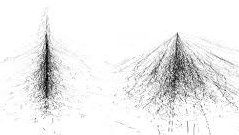
\includegraphics[width=0.8\textwidth]{figures/showers.png}
%	\caption{Comparison of a hadronic shower profile versus an electromagnetic shower profile}
%	\label{fig:showers}
%\end{figure}
%
\par To measure the energy of the primary particle, calorimeters are designed to contain the 
entire shower. Because of the clear differences between EM and hadronic showers, EM calorimeters 
are dedicated to containing EM showers while hadronic calorimeters are dedicated to containing 
hadronic showers. Both calorimeters could be {\it homogenous} or {\it sampling}. For the former, the shower is 
contained in a homogenous material that acts as both an absorber and an active medium where 
the shower is detected. The latter is made up of alternating layers of an absorber and active materials. 
One advantage that a sampling calorimeter 
has over a homogenous calorimeter is that the absorber and active materials can be 
optimized separately, allowing construction of a more compact calorimeter. The absorber 
could be made of a very dense material such as \ch{Fe}, \ch{Pb} or \ch{U}, while the active 
material could be made of liquid \ch{Ar} or \ch{Si} detectors. Since only a part of the shower is 
detected, the energy resolution in a sampling calorimeter is usually lower than in 
a homogenous calorimeter. 

\par The ATLAS calorimeter system~\cite{Puzo2002340} is made up of a dedicated set of sampling calorimeters that cover 
up to $|\eta|<4.9$. These calorimeters are can be grouped into the Liquid 
\ch{Ar} Calorimeter~\cite{LARG-2009-01} (LAr) and the Tile Calorimeter~\cite{TCAL-2010-01},
 where the Tile Calorimeter is designed to contain hadronic particle
 showers and the Lar Calorimeter has dedicated components 
for both hadronic and EM particle showers. 
%Figure~\ref{fig:caloSketch} shows a sketch 
%of these segments. 
%
%\begin{figure}[!h]
%	\centering
%   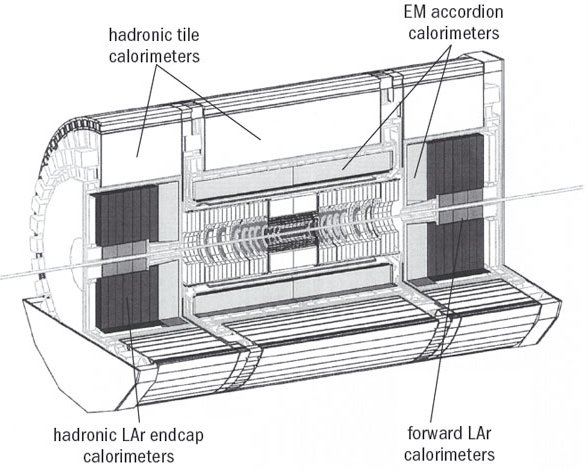
\includegraphics[width=0.8\textwidth]{figures/caloSketch.jpg}
%	\caption{A cutaway view of the ATLAS calorimeter system}
%	\label{fig:caloSketch}
%\end{figure}
%
\subsubsection{Liquid Argon Calorimeter}
\par As show in Figure~\ref{fig:larCal} the LAr Cal is made up of the Electromagnetic Calorimeter (EM Cal), the 
hadronic end-cap (HEC) and the forward calorimeter (FCAL). For most of the LAr the
 absorber material is \ch{Pb}, held in place by a thin layer of stainless steel and molded into 
an accordion shape. In parts of the FCAL and the HEC \ch{Pb} is replaced by \ch{Cu}
 and \ch{W} as the absorber material to accommodate higher particle rates. 
The active material in all components is liquid \ch{Ar}, filled in 
between \ch{Pb}, \ch{Cu} or \ch{W} to a \SI{2}{\mm} width. Electrode boards that are molded 
into accordion shapes are placed inside the liquid \ch{Ar} to collect electrons 
from the particle showers. These electrons are amplified and constitute signal.
 
\par The barrel component of the EM Cal is made up of two half wheels that are each made up of 1024 absorber sheets.
It covers up to $|\eta|<1.475$ and $r<22 X_0$. A \SI{1}{\cm} thick liquid \ch{Ar} region with 
electrodes perpendicular to the beam axis is at the innermost surface of the barrel EM Cal to 
act as a presampler. A cell is defined in $\eta$ by etching the electrode boards and in $\phi$ by 
grouping 4 electrode boards. Overall, the EM Cal end-caps cover $1.375<|\eta|<3.2$. 
Each end-cap is made up of to concentric wheels. The inner wheel has 256 absorbers and 
the outer wheel has 768 absorbers. The presampler for this region 
is similar to the barrel region except that it is \SI{5}{\mm} thick. The copper absorbers in the 
HEC are \SI{25}{\mm} thick, interleaved with \SI{7.4}{mm} thick liquid \ch{Ar}. 
The FCal on the other hand is made of 3 levels. The first 
level is of \ch{Cu} absorbers and the other two levels are made of \ch{W} absorbers.  
All the other components in the FCal are the same as in the EM Cal.

\begin{figure}[!h]
	\centering
   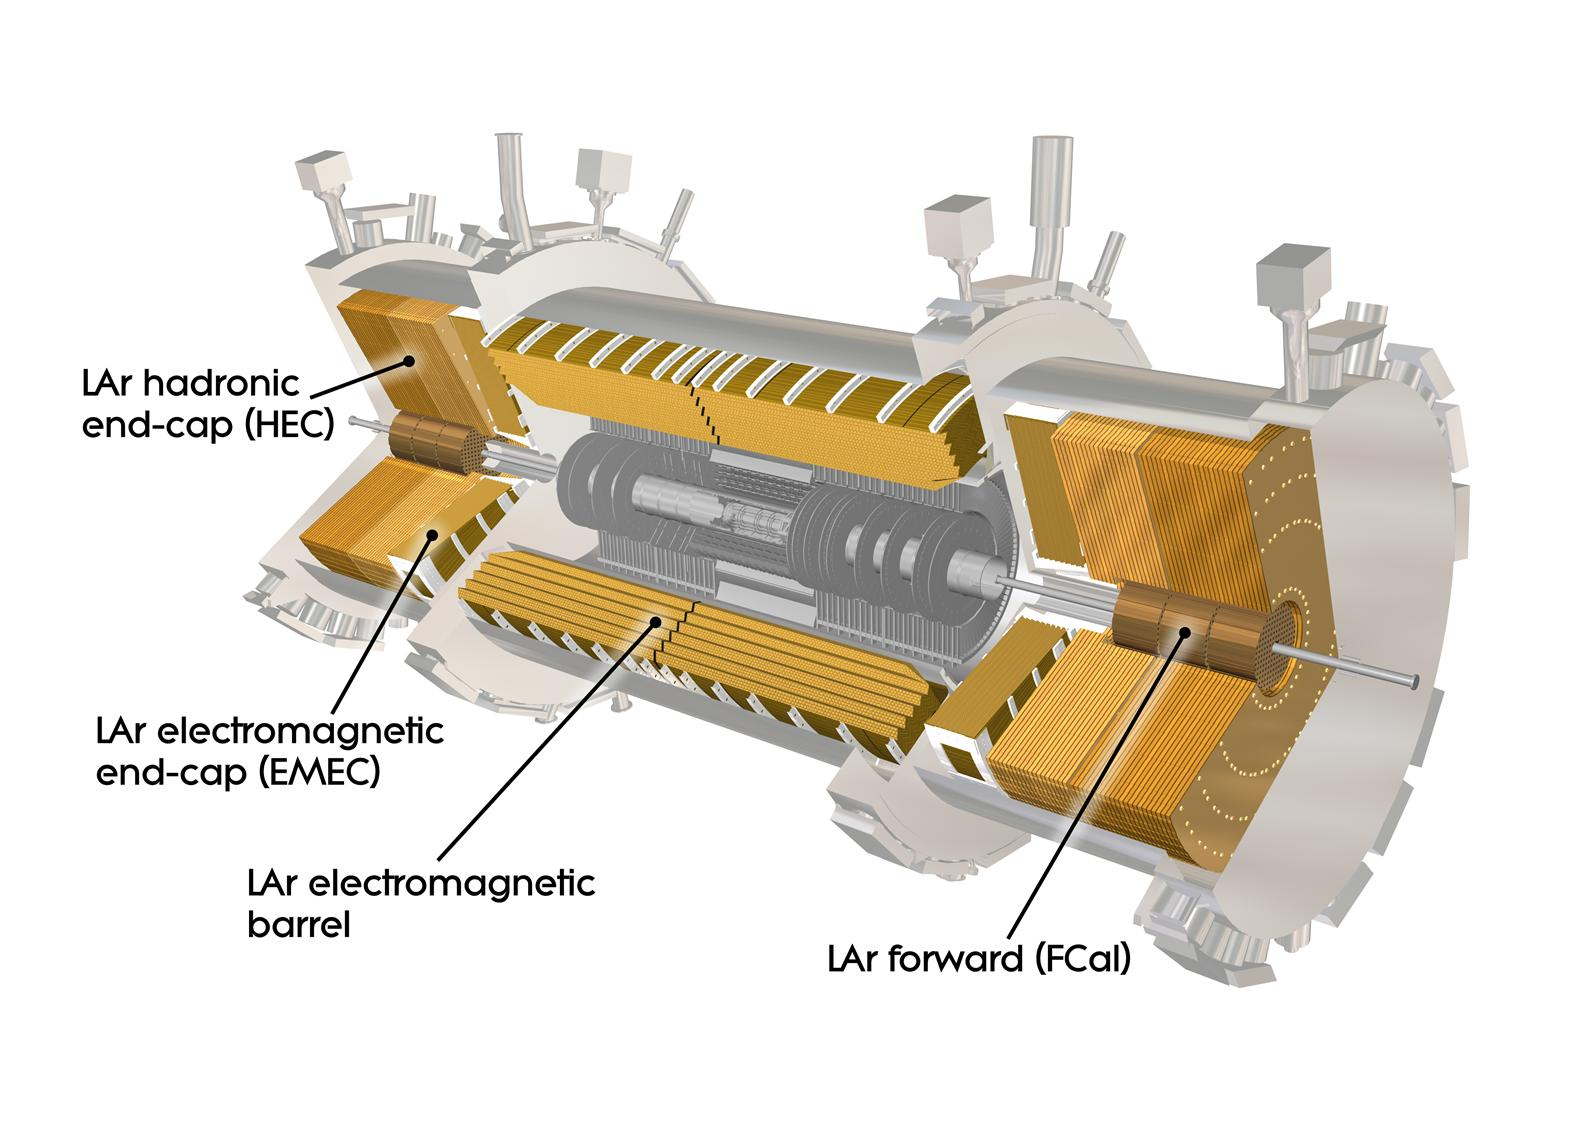
\includegraphics[width=0.8\textwidth]{figures/larCal.jpg}
	\caption{A cutaway view of the ATLAS calorimeter system}
	\label{fig:larCal}
\end{figure}

\subsubsection{Tile Calorimeter}
\par The largest calorimeter in ATLAS is the Tile Cal, shown in Figure~\ref{fig:larCal},
  covering up to $|\eta|<1.7$. It is placed 
just outside the LAr Calorimeter, with an inner radius of \SI{2.28}{\m}  and an outer 
radius of \SI{4.25}{\m}. It is split into a barrel region and an two {\it extended}
regions that align with the Lar end-caps. The barrel and extended components each comprise 64 modules.
 Each module is made up of \SI{5}{\mm} thick \ch{Fe} absorbers 
interleaved with \SI{3}{\mm} scintillating tiles. This structure makes a wedge shaped module 
that has a width $\Delta\phi=0.1$. A picture of one such module is shown in Figure~\ref{fig:tileCalmodule}.
Readout fibres are placed at the edges of each scintillating tile to collecting photons as signal. These 
fibres are then grouped at the edge of each module and connected to a photomultiplier, 
which multiplies the collected photons to make a detectable signal. The fibres are visible at the bottom 
of the picture in Figure~\ref{fig:tileCalmodule}. 

\begin{figure}[!h]
	\centering
   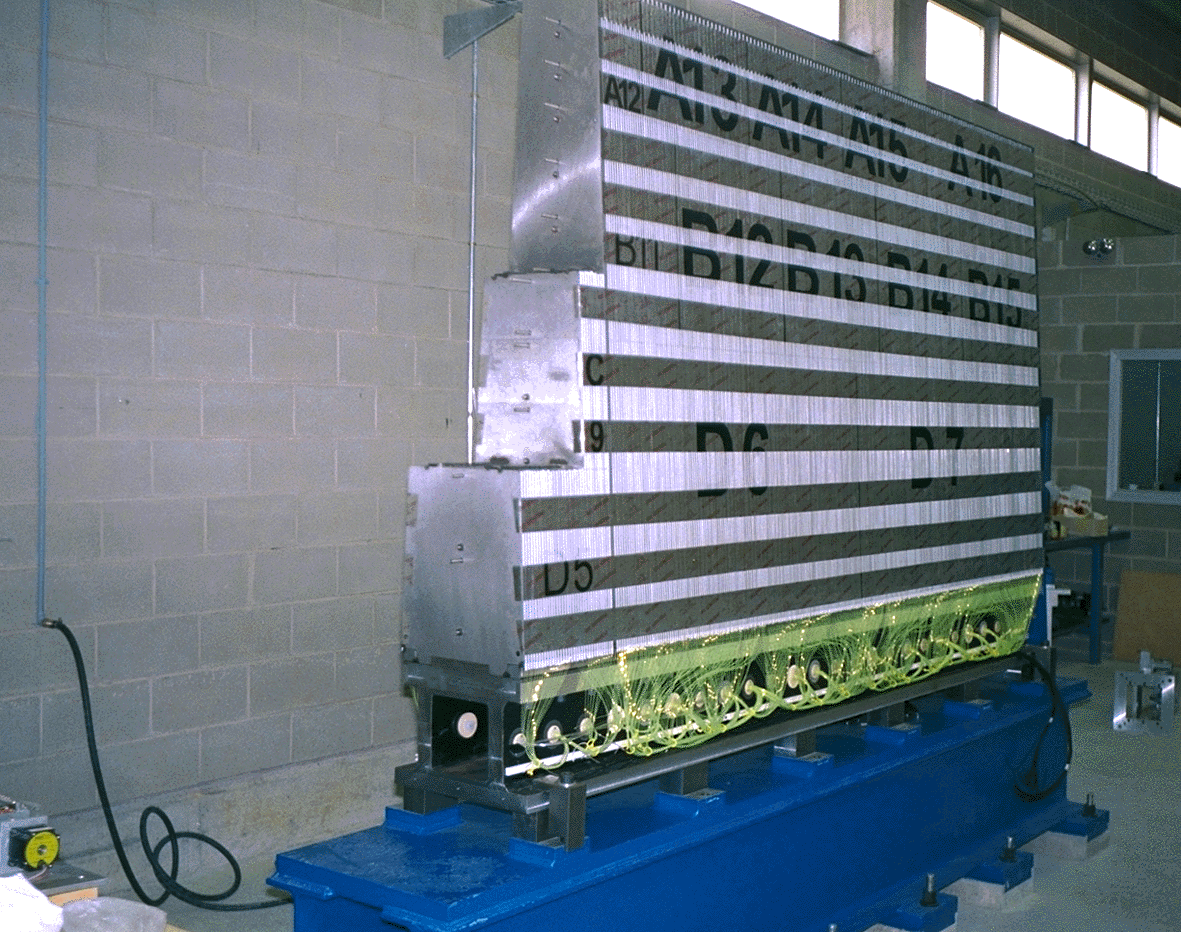
\includegraphics[width=0.8\textwidth]{figures/tileCalmodule.png}
	\caption{A photograph of a Tile Calorimeter module}
	\label{fig:tileCalmodule}
\end{figure}
